\documentclass{article}
	\usepackage{amsmath}
	\usepackage{bm}
	\usepackage{graphicx}
	\usepackage{mhchem}
	\usepackage{subcaption}
	\usepackage[margin=1cm]{caption}
	\usepackage{amssymb}
	\newcommand{\sumc}[1]{\sum_{c=1}^N \mu_c N_c^#1}
  \renewcommand{\d}{\mathrm{d}} 
  \newcommand{\matr}[1]{\bm{#1}}
  \newcommand{\dOne}[2]{\frac{\d#1}{\d#2}}
  \newcommand{\pOne}[2]{\frac{\partial#1}{\partial#2}}
  \newcommand{\note}[1]{\\\textbf{\textit{Note: }}#1\\\\}
	\date{3 September, 2015}
	\author{J. Mann}
	\title{Day 3 Notes}
	\date{September 3, 2015}
	\graphicspath{{Day3NotesPics/}}
\begin{document}
\maketitle{}
\begin{section}{Intro}
  One fundamental formula for surfaces \& adsorption is the differential 1-form
  \begin{align}
    -d\gamma = \bar{S} dT - \tau dP + \sum_{n=1}^e \Gamma_n d\mu_n
    \label{Eq:differential 1-form}
  \end{align}
  Where $\bar{S}, \tau, \{ \Gamma_c\}$ are excess quantities.
  
  A second  formula is the Gibbs' phase rule
 \begin{align}
 f = c - p + 2    
    \label{Eq:Gibbs Phase Rule}
  \end{align}

  \eqref{Eq:Gibbs Phase Rule} requires that \underline{any two} of the excess must be set to zero. That determines the ``Convention''. The lecture today will start from this point. 
  
  \begin{itemize}
    \item The ``Gibbs convention'' $\tau = 0, \Gamma_1 = 0$
    \item The ``Hansen convention'' $\Gamma_1 = 0, \Gamma_2 = 0$
  \end{itemize}

\end{section}
\begin{section}{Surface excess entropy}
	\begin{align*}
		\bar{S}\times \matr{A} \equiv S^s
	\end{align*}
  \begin{itemize}
    \item $\bar{S}$ is intensive, $S^s$ is extensive.
    \item Surface excess entropy is defined using $\lambda_1$ and $\lambda_2$ determined with \eqref{Eq:differential 1-form}.
    \item Be sure to tell the reader the convention you're using!
  \end{itemize}
  Also 
  \begin{align*}
	  \tau\times \matr{A} &\equiv V^s \text{Volume Excess}\\
	  \Gamma_c\times \matr{A} &\equiv N_c^s \text{Mole Number Excess}\\
    U &= ST - PV + \sum_{c=1}^N \mu_c N + \gamma A\\
    \check{U}^{+} &= \check S^{+}T - P + \sum_{c=1}^N \mu_c \check N^{+}\\
    \check{U}^{-} &= \check S^{-}T - P + \sum_{c=1}^N \mu_c \check N^{-}\\
    U^s &= U - \lambda^{+}\check U^{+} -\lambda^{-} \check U^{-} \text{similar for }S^s\text{, etc.}\\
    \therefore U^s &= S^s T - P V^s + \sum_{c=1}^N \mu_c N^s + \gamma A
  \end{align*}
  \note{$F$ is the Helmholtz Free Energy, typically defined in texts as $A$}
  Now to compute $\d U^s$. Recall that we know a 1-form for $-\d \gamma$ so that 
  \begin{align*}
    dU^s &= T dS^s - P dV^s + \sum_{c=1}^N \mu_c \d N_c^s + \gamma \d A\\
  \end{align*}

  Now recall the Euler Integral theorem to find 
  \begin{align*}
    U^s = TS^s - P \d V^s + \sumc + \gamma A
    H^s &\equiv U^s + PV^s\\
    F^s &\equiv U^s - TS^s\\
    \d F^s &= - S^s \d T - P\d V^s + \sum_{c=2}^{\#\mathrm{components}} \mu_c\d N_c^s + \gamma \d A
  \end{align*}
  If $T$ is constant, $\d T = 0$, and in the Gibbs convention, $V^s = 0$, and $N_1^s =0$. Also if the composition is constant, $\d N_2^s = 0, \d N_3^s = 0,\ldots$ Then
  \begin{align*}
    \d F^s = \gamma \d A
  \end{align*} (Here $\gamma$ is the Helmholtz free Energy per Area $\gamma = \pOne{F}{Area}$)
\begin{subsection}{Some Details}
  \begin{align*}
    F^s &= U^s - TS^s\\
    \d F^s &= \d U^s - T dS^s - S^s \d T
  \end{align*}
  You have a differential 1-form for $\d U^s$, upon substitution $+T\d S^s$ adds out the $-T\d S^s$ term.
  \begin{align*}
    \d U^s &= T \d S^s - P \d V^s + \sum_{i=1}^N \mu_c \d N_c^s + \gamma \d A\\
    H^s &= U^s + PV^s \\
    F^s &= U^s - TS^s \\
    \d F^s &= -S^s \d T - p \d V^s
    \label{Basic definitions}
  \end{align*}
  If T is constant and the mole numbers are constant, $\d T = 0$, $\d N_c^s = 0$, assume Gibbs convention $V^s = 0$. Then $dF^s = \gamma \d A$ Here $\gamma$ is Helmholtz free energy per unit area
\end{subsection}
\end{section}
\begin{section}{Concentration and Surface Tension}
\begin{align*}
	-\d \gamma &= \bar{S}\d T - \tau\d P + \Gamma_\ce{H2O}\d\mu_\ce{H2O} + \Gamma_s\d\mu_s\\
\end{align*}
Assume $p$ is constant
\begin{align*}
	\tau = 0, \Gamma_\ce{H2O} &= 0\text{ (Gibbs Convention)}\\
	\d T&=0\\
	\text{then}\\
	-\d \gamma &= \Gamma_s\d\mu_s\\
	\Gamma_s &= -\pOne{\gamma}{\mu_s}\\
	\mu_s &= \mu^{\circ}_s + k_B T\ln{(a_s)}\\
	a_s &= \alpha C_s
\end{align*}
  $\gamma, \nu$ constant.???

\end{section}
\begin{section}{How to find a derivative given noisy function}
At some point you will be taking experimental $\gamma$ vs $C$ data and estimating $\pOne{\gamma}{\ln{(C)}}$ - how to do this keeping in mind that there is always some error associated with measuring $\gamma$ is a point of interest.
  Suppose you know that a smooth formula works well in representing your data.
	
	$y = f(x)$ so that $ \dOne{y}{x} = f^\prime (x)$ is smooth in the sense that
	\begin{align*}
		f^\prime(x) = \lim_{h\rightarrow 0}{\frac{(f(x-h) - f(x))}{h}}
	\end{align*} exists at each point $x$.

	Now do a measurement and find that there is experimental error at each point so that 
$y = f(x) + \epsilon(x)$ where $\epsilon$ is a random number from the uncertainty of the measurement.

\begin{align*}
\dOne{y}{x} &= f(x) + \epsilon(x)\\
\epsilon^\prime(x) &= \lim_{h\rightarrow 0} \frac{\epsilon(x-h)-\epsilon(x)}{h} \text{ (In general, does not exist!)}
\end{align*}
\end{section}
\begin{section}{Gibbs Approach}

	\begin{figure}[h]
		\centering
		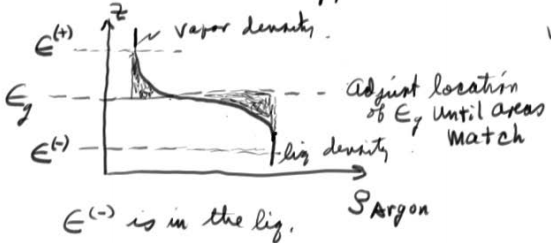
\includegraphics[height=100pt]{GibbsApproach}
		\caption{A system of liquid and vapor Argon. The vertical axis is distance normal to the surface, and the horizontal axis is density of Argon, $\rho_\text{Argon}$. The density is constant at some distance from the interface, then changes (following a hyperbolic tangent curve) as the interface is approached. $\varepsilon_g$ is defined as the line where the areas (above and below the curve) match.}
		\label{fig:Gibbs Surface Level}
	\end{figure}
	Consider the gibbs approach. Define $\varepsilon^+$ as the vapor, $\varepsilon^-$ as the liquid (as in Figure~\ref{fig:Gibbs Surface Level}). These are the two asymptotes of a hyperbolic tangent curve. Then we will have $\rho^z - \rho^+ \geq 0$ for $z$ in the range of tanh curve.
	Similarly $\rho^z - \rho^- \leq 0$ for $z$ in the same range.

	\begin{align*}\Gamma \equiv \int_{\varepsilon_g}^{\varepsilon^+}( \rho^z - \rho^+ )\d z + \int_{\varepsilon^-}^{\varepsilon^g}( \rho^z - \rho^-) \d z
	\end{align*}

	Now then: $\Gamma_1 = 0$ therefore, excess of the major component is 0.

	More generally,
	\begin{align*}
		\Gamma_c = \int_{\varepsilon^-}^{\varepsilon^g}(\rho_c(z) - \rho_c^-)\d z + \int_{\varepsilon_g}^{\varepsilon+} (\rho_c(z) - \rho_c^+)\d z
	\end{align*}
	if $\Gamma_1 = 0$ then there is some $\varepsilon_g$ such that in/out $\Gamma_1 = 0$. By correlation, this fixes the location of the gibbs surface at $\varepsilon_g$. 

	However, $\Gamma_c, c\neq 0$ may be either $\Gamma_c > 0$ or $\Gamma_c < 0$, although for the usual surfactants, $\Gamma_c > 0$.
	\begin{figure}[h]
		\centering
		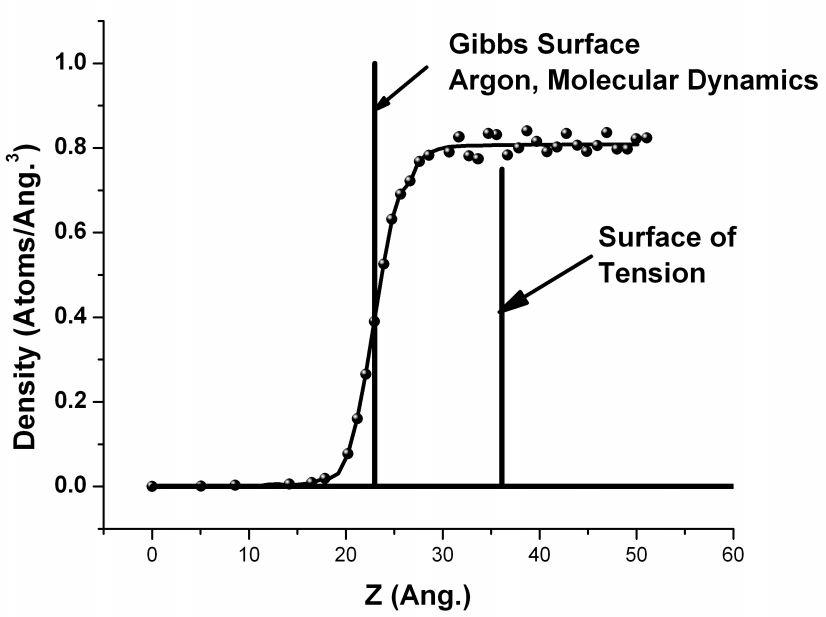
\includegraphics[height=150pt]{GibbsSurface}
		\caption{Work done by Mann wih MD simulation showing the agreement with a tanh curve, and showing the Gibbs Surface of Argon.}
		\label{fig:Gibbs Surface Detail}
	\end{figure}
\end{section}
\begin{section}{}
	\begin{figure}[h]
		\centering
		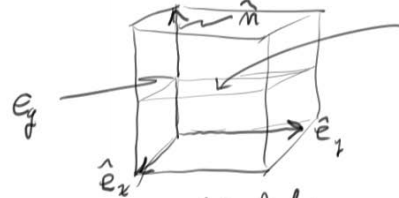
\includegraphics[height=100pt]{GibbsSurfaceToEg}
		\caption{Gibbs Surface Corresponding to $\varepsilon_g$}
		\label{fig:Gibbs Surface EgBox}
	\end{figure}
	With this definition, $\Gamma_{c(c\neq 1)} = \int_{-\infty}^{+\infty} \rho_c(z) - \rho_c^(\pm) ) dz$

	$+, - $ are the two phases with density $\rho_c^+, \rho_c^-$
	Only for $c=1$ does $\Gamma_1 = 0$ which determines the rest of the excess. Also in the Gibbs convention, 
	\center{\boxed{V_{\mathrm{total}} = V^+ + V^-}}

\end{section}

\begin{section}{The Case of Curved Surfaces}
	\begin{figure}[h]
		\centering
		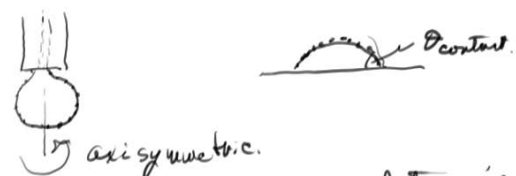
\includegraphics[height=60pt]{pendantDrop}
		\caption{The pendant drop method. This method is axisymmetric, and takes advantage of the fact that the contact angle of a drop on a surface, $\theta$, is a constant.}
		\label{fig:pendant drop}
	\end{figure}

	To determine the surface tension - you determine the boundary function, then fit it to a model. You need the relationship between the surface tension, the local radii of curvature, and thee pressure drop \underline{across} the interface - the jump of the pressure.
	\begin{figure}[h]
		\centering
		\begin{subfigure}[t]{0.4\textwidth}
			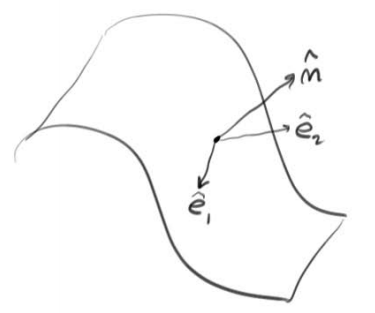
\includegraphics[height=100pt]{generalSurface}
			\caption{Some surface}
		\end{subfigure}
		\begin{subfigure}[t]{0.4\textwidth}
			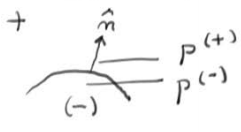
\includegraphics[height=50pt]{curvedSurface}
			\caption{\\$P^+$ is the pressure in the $+$ phase\\	
			$P^-$ is the pressure in the $-$ phase}
		\end{subfigure}
		\caption{A generic curved surface. $\hat{e}_1,\hat{e}_2$ are tangent to the surface, making $\hat{n} = \hat{e}_1\times\hat{e}_2$ normal to the surface, provided $\hat{e}_1\neq\hat{e}_2$}
		\label{fig:surface}
	\end{figure}
	Consider Figure~\ref{fig:surface}. Anywhere on the curved surface of the phase, you can construct a normal. What you have to think about is the pressure drop across this interface. That is the jump in the pressure as you approach the interface 
	\begin{align*}
		[P] \equiv \lim_{z\downarrow \mathrm{surface}}{( P^{+})} - \lim_{z\uparrow \mathrm{surface}}{( P^{-})}
	\end{align*}.
\end{section}

\end{document}
